\documentclass[12pt]{beamer}
\usepackage[utf8]{inputenc}
\usepackage[T1]{fontenc}
\usepackage{lmodern}
\usepackage[spanish]{babel}
\usepackage{graphicx}
\usepackage{ragged2e} %to use \justify
\usetheme{Rochester}
\title{Coloquio de Modalidades 2018-2}
\subtitle{Ayudantía Docente en Programación}
\author{Alumno: José Armando Gutiérrez Núñez\\Maestro: Thelma Violeta Ocegueda Miramontes}
\logo{
\includegraphics[scale=0.07]{uabclogo.PNG}}
\institute[U.A.B.C.]{Universidad Autónoma de Baja California}
\date{}
\setbeamercovered{transparent}


\begin{document}
    \frame{\titlepage}
    
    %***********************************************************
    %*                      COMPETENCIA                        *
    %***********************************************************
    %- - - - - - - - - - - SLIDE 01 - - - - - - - - - - - - - - - -    
    \begin{frame}{Competencia}
    \justify
    \hspace{5mm}Elaborar material didactico, como ejemplos y ayudas visuales, utilizando las tecnologías de la información, para enriquecer y facilitar la enseñanza de la lógica y la programación con responsabilidad y perseverancia.
    \end{frame}
    \begin{frame}[t]{Actividades}
        \begin{center}
            \textbf{Algunas actividades}
        \end{center}
        \begin{block}{Presentaciones}
            Elaborar presentaciones en latex de los apuntes de la materia.
        \end{block}
        \begin{block}{Código Ejemplos}
            Elaborar ejemplos de código, donde una parte del código esté mal y los alumnos tengan que identificar el error.
        \end{block}
    \end{frame}


    %***********************************************************
    %*                      ACTIVIDADES                        *
    %***********************************************************
    %- - - - - - - - - - - SLIDE 02 - - - - - - - - - - - - - - - -
    \begin{frame}{Actividades}
    \begin{center}
        {\large \textbf{De las presentaciones}}
    \end{center}
        \justify
        \hspace{5mm}Elaboración de presentaciónes utilizando, utilizando bibliografía actual.
        Asegurando que la información que se transmite al alumno es la mas actual, o mitiendo detalles que han quedado obsoletos con el tiempo.
    \end{frame}


    %- - - - - - - - - - - SLIDE 03 - - - - - - - - - - - - - - - -
    \begin{frame}{Actividades}
        \begin{center}
            {\large \textbf{Del software utilizado}}
        \end{center}
        \justify
        \hspace{5mm}Elaboracion de las presentaciones en Latex, asegurando portabilidad del documento final, evitando con ello errores al visualizarla en diferentes dispositivos.
        Facilidad de edición, ya que al efectuar un cambio en algun tema, no se requiere buscar entre todo el ducumento, ya que permite dividir secciones en archivos separados.
    \end{frame}


    %***********************************************************
    %*                      EJEMPLOS                           *
    %***********************************************************
    %- - - - - - - - - - - SLIDE 04 - - - - - - - - - - - - - - - -
    \begin{frame}{Ejemplo de Presentacion}
       \begin{columns}
           \begin{column}{0.5 \textwidth}
               \fcolorbox{blue}{white}{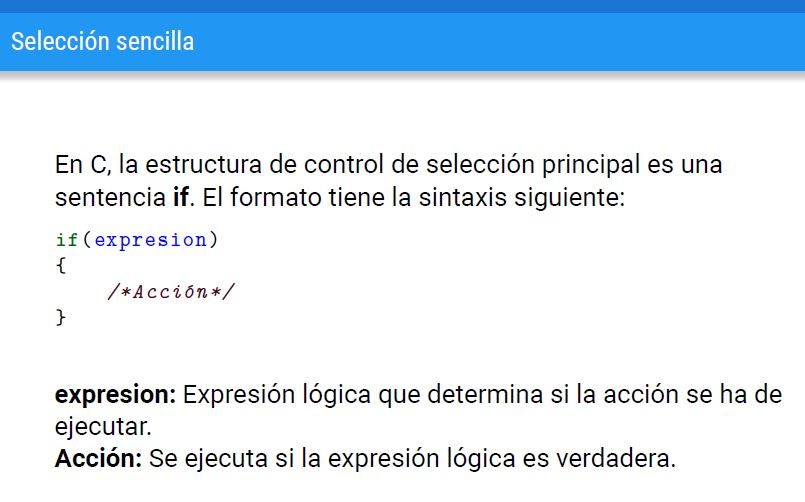
\includegraphics[scale=0.26]{explicacionIf.JPG}}
           \end{column}
           \begin{column}{0.5 \textwidth}
                \fcolorbox{blue}{white}{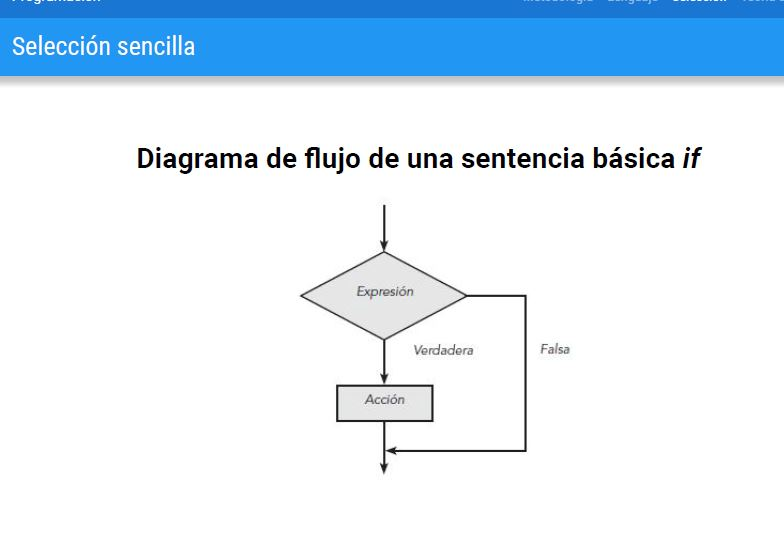
\includegraphics[scale=0.24]{diagramaIf.JPG}}
           \end{column}
       \end{columns}
    \end{frame}


    %- - - - - - - - - - - SLIDE 05 - - - - - - - - - - - - - - - -
    \begin{frame}{Ejemplo de Presentacion}
        \begin{columns}
            \begin{column}{0.5 \textwidth}
                \fcolorbox{blue}{white}{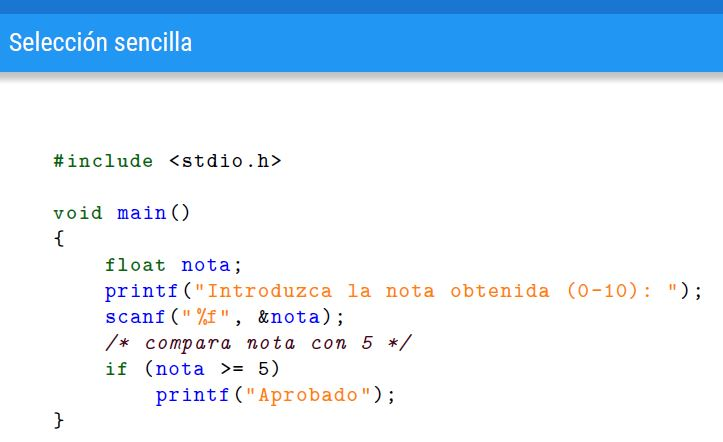
\includegraphics[scale=0.29]{ejemploIf.JPG}}
            \end{column}
            \begin{column}{0.5 \textwidth}
                \fcolorbox{blue}{white}{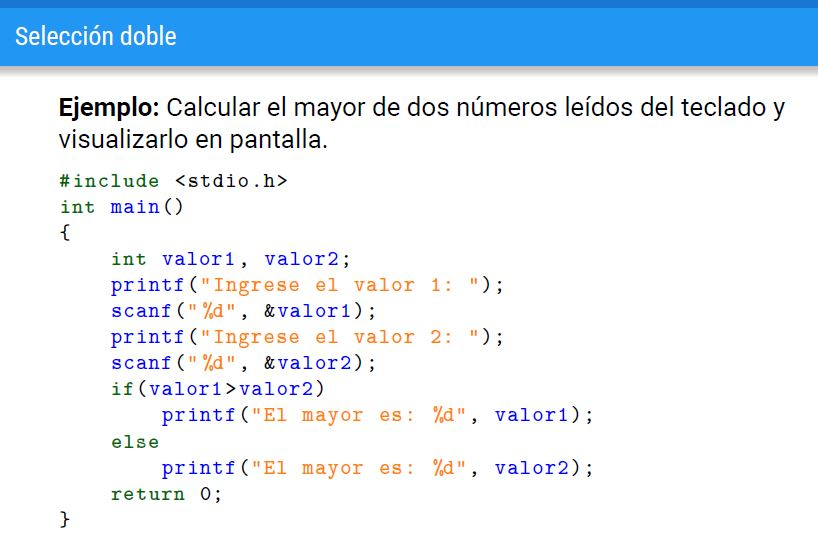
\includegraphics[scale=0.24]{ejemploIfElse.JPG}}
            \end{column}
        \end{columns}
    \end{frame}


    %************************************************************
    %*                  APLICACION DE CONOCIMIENTOS             *
    %************************************************************
    %- - - - - - - - - - - SLIDE 06 - - - - - - - - - - - - - - - -
    \begin{frame}{Aplicación de conocimientos}
        \begin{center}
            \textbf{Aplicación de los conocimientos adquiridos  en la carrera}
        \end{center}
        \hspace{5mm}Durante la ayudantía pude aplicar conocimientos adquiridos en asignaturas tales como Programación y Elaboración de Documentación Técnica.\\              
        \hspace{5mm}Programación que es una actividad cotidiana y que semestre a semestre se ha ido mejorando la técnica, gracias a los maestros designados, desde un inició en el que básicamente se nos enseña a usar un ambiente integrado de desarrollo para solamente aprender a conocer la sintaxis y alguna reglas básicas, hasta en aquellas asignaturas en las que la exigencia es alta.
    \end{frame}


    %***********************************************************
    %*                      APRENDIZAJE                        *
    %***********************************************************
    %- - - - - - - - - - - SLIDE 07 - - - - - - - - - - - - - - - -
    \begin{frame}{Enseñanza Académica y Experiencia Personal}
        Como enseñanza académica, esta actividad ayuda a reafirmar conocimientos básicos.
        \\
        \hspace{5mm}Programación, que siendo una actividad cotidiana, siempre está en evolución, en este orden de ideas, comprender que algunas prácticas evolucionan, ya sea eliminando y agregando o simplemente modificando detalles simples.\\
        \hspace{5mm}Como enseñanza personal, fue poder aportar un poco a lo mucho que la universidad me ha ofrecido a través del tiempo. Aportando algo tal vez simbólico, pero siempre es bueno retribuir por todo lo que me ha ofrecido.
    \end{frame}
    
    \begin{frame}
        \begin{center}
            \textcolor{blue}{\Huge \textbf{GRACIAS!}}
        \end{center}
    \end{frame}

\end{document}